% Options for packages loaded elsewhere
\PassOptionsToPackage{unicode}{hyperref}
\PassOptionsToPackage{hyphens}{url}
%
\documentclass[
]{article}
\usepackage{lmodern}
\usepackage{amsmath}
\usepackage{ifxetex,ifluatex}
\ifnum 0\ifxetex 1\fi\ifluatex 1\fi=0 % if pdftex
  \usepackage[T1]{fontenc}
  \usepackage[utf8]{inputenc}
  \usepackage{textcomp} % provide euro and other symbols
  \usepackage{amssymb}
\else % if luatex or xetex
  \usepackage{unicode-math}
  \defaultfontfeatures{Scale=MatchLowercase}
  \defaultfontfeatures[\rmfamily]{Ligatures=TeX,Scale=1}
\fi
% Use upquote if available, for straight quotes in verbatim environments
\IfFileExists{upquote.sty}{\usepackage{upquote}}{}
\IfFileExists{microtype.sty}{% use microtype if available
  \usepackage[]{microtype}
  \UseMicrotypeSet[protrusion]{basicmath} % disable protrusion for tt fonts
}{}
\makeatletter
\@ifundefined{KOMAClassName}{% if non-KOMA class
  \IfFileExists{parskip.sty}{%
    \usepackage{parskip}
  }{% else
    \setlength{\parindent}{0pt}
    \setlength{\parskip}{6pt plus 2pt minus 1pt}}
}{% if KOMA class
  \KOMAoptions{parskip=half}}
\makeatother
\usepackage{xcolor}
\IfFileExists{xurl.sty}{\usepackage{xurl}}{} % add URL line breaks if available
\IfFileExists{bookmark.sty}{\usepackage{bookmark}}{\usepackage{hyperref}}
\hypersetup{
  pdftitle={Gestion de Portefeuille},
  hidelinks,
  pdfcreator={LaTeX via pandoc}}
\urlstyle{same} % disable monospaced font for URLs
\usepackage[margin=1in]{geometry}
\usepackage{color}
\usepackage{fancyvrb}
\newcommand{\VerbBar}{|}
\newcommand{\VERB}{\Verb[commandchars=\\\{\}]}
\DefineVerbatimEnvironment{Highlighting}{Verbatim}{commandchars=\\\{\}}
% Add ',fontsize=\small' for more characters per line
\usepackage{framed}
\definecolor{shadecolor}{RGB}{248,248,248}
\newenvironment{Shaded}{\begin{snugshade}}{\end{snugshade}}
\newcommand{\AlertTok}[1]{\textcolor[rgb]{0.94,0.16,0.16}{#1}}
\newcommand{\AnnotationTok}[1]{\textcolor[rgb]{0.56,0.35,0.01}{\textbf{\textit{#1}}}}
\newcommand{\AttributeTok}[1]{\textcolor[rgb]{0.77,0.63,0.00}{#1}}
\newcommand{\BaseNTok}[1]{\textcolor[rgb]{0.00,0.00,0.81}{#1}}
\newcommand{\BuiltInTok}[1]{#1}
\newcommand{\CharTok}[1]{\textcolor[rgb]{0.31,0.60,0.02}{#1}}
\newcommand{\CommentTok}[1]{\textcolor[rgb]{0.56,0.35,0.01}{\textit{#1}}}
\newcommand{\CommentVarTok}[1]{\textcolor[rgb]{0.56,0.35,0.01}{\textbf{\textit{#1}}}}
\newcommand{\ConstantTok}[1]{\textcolor[rgb]{0.00,0.00,0.00}{#1}}
\newcommand{\ControlFlowTok}[1]{\textcolor[rgb]{0.13,0.29,0.53}{\textbf{#1}}}
\newcommand{\DataTypeTok}[1]{\textcolor[rgb]{0.13,0.29,0.53}{#1}}
\newcommand{\DecValTok}[1]{\textcolor[rgb]{0.00,0.00,0.81}{#1}}
\newcommand{\DocumentationTok}[1]{\textcolor[rgb]{0.56,0.35,0.01}{\textbf{\textit{#1}}}}
\newcommand{\ErrorTok}[1]{\textcolor[rgb]{0.64,0.00,0.00}{\textbf{#1}}}
\newcommand{\ExtensionTok}[1]{#1}
\newcommand{\FloatTok}[1]{\textcolor[rgb]{0.00,0.00,0.81}{#1}}
\newcommand{\FunctionTok}[1]{\textcolor[rgb]{0.00,0.00,0.00}{#1}}
\newcommand{\ImportTok}[1]{#1}
\newcommand{\InformationTok}[1]{\textcolor[rgb]{0.56,0.35,0.01}{\textbf{\textit{#1}}}}
\newcommand{\KeywordTok}[1]{\textcolor[rgb]{0.13,0.29,0.53}{\textbf{#1}}}
\newcommand{\NormalTok}[1]{#1}
\newcommand{\OperatorTok}[1]{\textcolor[rgb]{0.81,0.36,0.00}{\textbf{#1}}}
\newcommand{\OtherTok}[1]{\textcolor[rgb]{0.56,0.35,0.01}{#1}}
\newcommand{\PreprocessorTok}[1]{\textcolor[rgb]{0.56,0.35,0.01}{\textit{#1}}}
\newcommand{\RegionMarkerTok}[1]{#1}
\newcommand{\SpecialCharTok}[1]{\textcolor[rgb]{0.00,0.00,0.00}{#1}}
\newcommand{\SpecialStringTok}[1]{\textcolor[rgb]{0.31,0.60,0.02}{#1}}
\newcommand{\StringTok}[1]{\textcolor[rgb]{0.31,0.60,0.02}{#1}}
\newcommand{\VariableTok}[1]{\textcolor[rgb]{0.00,0.00,0.00}{#1}}
\newcommand{\VerbatimStringTok}[1]{\textcolor[rgb]{0.31,0.60,0.02}{#1}}
\newcommand{\WarningTok}[1]{\textcolor[rgb]{0.56,0.35,0.01}{\textbf{\textit{#1}}}}
\usepackage{graphicx}
\makeatletter
\def\maxwidth{\ifdim\Gin@nat@width>\linewidth\linewidth\else\Gin@nat@width\fi}
\def\maxheight{\ifdim\Gin@nat@height>\textheight\textheight\else\Gin@nat@height\fi}
\makeatother
% Scale images if necessary, so that they will not overflow the page
% margins by default, and it is still possible to overwrite the defaults
% using explicit options in \includegraphics[width, height, ...]{}
\setkeys{Gin}{width=\maxwidth,height=\maxheight,keepaspectratio}
% Set default figure placement to htbp
\makeatletter
\def\fps@figure{htbp}
\makeatother
\setlength{\emergencystretch}{3em} % prevent overfull lines
\providecommand{\tightlist}{%
  \setlength{\itemsep}{0pt}\setlength{\parskip}{0pt}}
\setcounter{secnumdepth}{-\maxdimen} % remove section numbering
\usepackage[utf8]{inputenc}
\usepackage{amsmath}
\usepackage{amsfonts}
\usepackage{amssymb}
\usepackage[cyr]{aeguill}
\usepackage[french]{babel}
\ifluatex
  \usepackage{selnolig}  % disable illegal ligatures
\fi

\title{Gestion de Portefeuille}
\usepackage{etoolbox}
\makeatletter
\providecommand{\subtitle}[1]{% add subtitle to \maketitle
  \apptocmd{\@title}{\par {\large #1 \par}}{}{}
}
\makeatother
\subtitle{TP-1: Analyse du CAC40}
\author{}
\date{\vspace{-2.5em}Février-Mars 2021}

\begin{document}
\maketitle

\hypertarget{les-donnuxe9es}{%
\subsection{Les données}\label{les-donnuxe9es}}

On charge les séries de rendements pour l'indice et les composants de
l'indice.

\begin{Shaded}
\begin{Highlighting}[]
\NormalTok{tickers }\OtherTok{\textless{}{-}} \ConstantTok{NULL}
\NormalTok{  ts.all }\OtherTok{\textless{}{-}} \FunctionTok{get.all.ts}\NormalTok{(}
    \StringTok{\textquotesingle{}CAC40\textquotesingle{}}\NormalTok{, tickers, }\AttributeTok{returns =} \ConstantTok{TRUE}\NormalTok{,}
    \AttributeTok{dt.start =} \FunctionTok{dmy}\NormalTok{(}\StringTok{\textquotesingle{}01Jul2007\textquotesingle{}}\NormalTok{), }\AttributeTok{combine =}\NormalTok{ T)}
  
  \CommentTok{\# remove Valeo {-} bad data}
\NormalTok{  ts.all }\OtherTok{\textless{}{-}}\NormalTok{ ts.all[,}\SpecialCharTok{{-}}\DecValTok{17}\NormalTok{]}
  
  \CommentTok{\# keep good data window}
\NormalTok{  ts.all }\OtherTok{\textless{}{-}} \FunctionTok{window}\NormalTok{(ts.all, }\FunctionTok{dmy}\NormalTok{(}\StringTok{\textquotesingle{}01Jul2007\textquotesingle{}}\NormalTok{), }
                   \FunctionTok{dmy}\NormalTok{(}\StringTok{\textquotesingle{}01Jan2009\textquotesingle{}}\NormalTok{))}
  
  \CommentTok{\# merge with cac40 index}
\NormalTok{  cac.index }\OtherTok{\textless{}{-}} \FunctionTok{get.ts}\NormalTok{(}\StringTok{\textquotesingle{}CAC40\textquotesingle{}}\NormalTok{, }\StringTok{\textquotesingle{}fchi\textquotesingle{}}\NormalTok{)}

\NormalTok{  cac.ret }\OtherTok{\textless{}{-}} \FunctionTok{returns}\NormalTok{(cac.index)}
  \FunctionTok{names}\NormalTok{(cac.ret) }\OtherTok{\textless{}{-}} \StringTok{\textquotesingle{}CAC40\textquotesingle{}}
\NormalTok{  ts.all }\OtherTok{\textless{}{-}} \FunctionTok{removeNA}\NormalTok{(}\FunctionTok{cbind}\NormalTok{(ts.all, cac.ret))}
\end{Highlighting}
\end{Shaded}

\begin{Shaded}
\begin{Highlighting}[]
\FunctionTok{plot}\NormalTok{(ts.all[, }\FunctionTok{c}\NormalTok{(}\DecValTok{1}\NormalTok{,}\DecValTok{2}\NormalTok{,}\DecValTok{3}\NormalTok{)], }\AttributeTok{main=}\StringTok{\textquotesingle{}Daily return\textquotesingle{}}\NormalTok{)}
\end{Highlighting}
\end{Shaded}

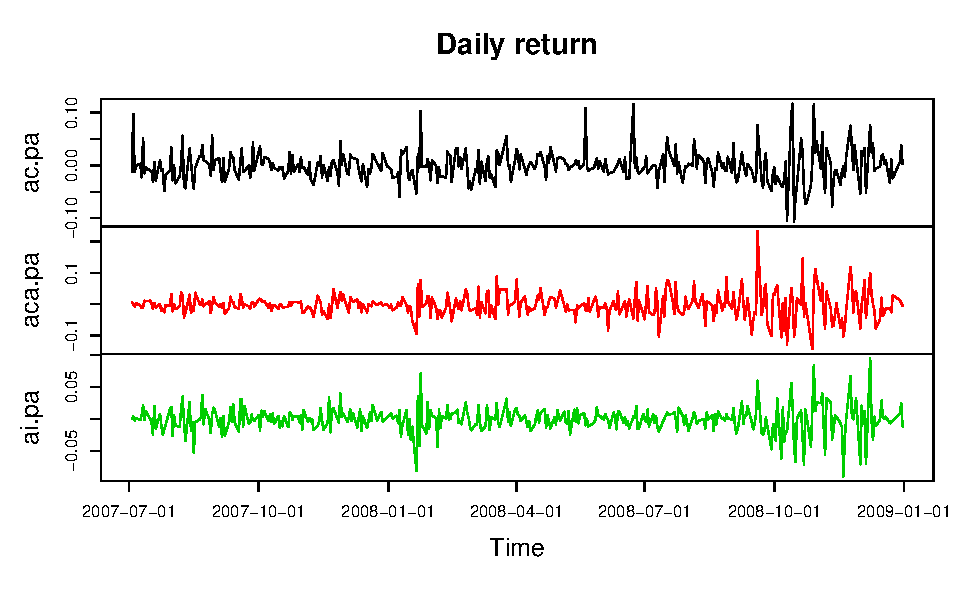
\includegraphics{TP1-Co_files/figure-latex/plot-cac-1-1.pdf}

Puis on filtre les points suspects: rendements supérieur à 8 s.d.

\begin{Shaded}
\begin{Highlighting}[]
  \CommentTok{\# flag bad data points: \textgreater{} * \textbackslash{}sigma}
\NormalTok{  good.limit }\OtherTok{\textless{}{-}} \DecValTok{8}\SpecialCharTok{*}\FunctionTok{apply}\NormalTok{(ts.all, }\DecValTok{2}\NormalTok{, sd)}
  
\NormalTok{  ts.bad }\OtherTok{\textless{}{-}}\NormalTok{ ts.all}\SpecialCharTok{*}\ConstantTok{FALSE}
  \ControlFlowTok{for}\NormalTok{(j }\ControlFlowTok{in} \FunctionTok{seq}\NormalTok{(}\FunctionTok{ncol}\NormalTok{(ts.bad))) \{}
\NormalTok{    ts.bad[,j] }\OtherTok{\textless{}{-}} \FunctionTok{abs}\NormalTok{(ts.all[,j]) }\SpecialCharTok{\textgreater{}}\NormalTok{ good.limit[j]}
\NormalTok{  \}}
\NormalTok{  good.index }\OtherTok{\textless{}{-}} \SpecialCharTok{!}\FunctionTok{apply}\NormalTok{(ts.bad,}\DecValTok{1}\NormalTok{,any)}
\NormalTok{  ts.all }\OtherTok{\textless{}{-}}\NormalTok{ ts.all[good.index,]}
\end{Highlighting}
\end{Shaded}

Finalement, on calcule les rendements hebdomadaires:

\begin{Shaded}
\begin{Highlighting}[]
  \CommentTok{\# aggregate returns by week}
\NormalTok{  by }\OtherTok{\textless{}{-}} \FunctionTok{timeSequence}\NormalTok{(}\AttributeTok{from=}\FunctionTok{start}\NormalTok{(ts.all), }
                     \AttributeTok{to=}\FunctionTok{end}\NormalTok{(ts.all), }\AttributeTok{by=}\StringTok{\textquotesingle{}week\textquotesingle{}}\NormalTok{)}
\NormalTok{  ts.all.weekly }\OtherTok{\textless{}{-}} \FunctionTok{aggregate}\NormalTok{(ts.all, by, sum)}

\NormalTok{  ts.stocks }\OtherTok{\textless{}{-}}\NormalTok{ ts.all.weekly[,}\SpecialCharTok{{-}}\DecValTok{40}\NormalTok{]}
\NormalTok{  ts.index }\OtherTok{\textless{}{-}}\NormalTok{ ts.all.weekly[,}\DecValTok{40}\NormalTok{]}
\end{Highlighting}
\end{Shaded}

\begin{Shaded}
\begin{Highlighting}[]
\FunctionTok{plot}\NormalTok{(ts.index, }\AttributeTok{main=}\StringTok{\textquotesingle{}Weekly return\textquotesingle{}}\NormalTok{)}
\end{Highlighting}
\end{Shaded}

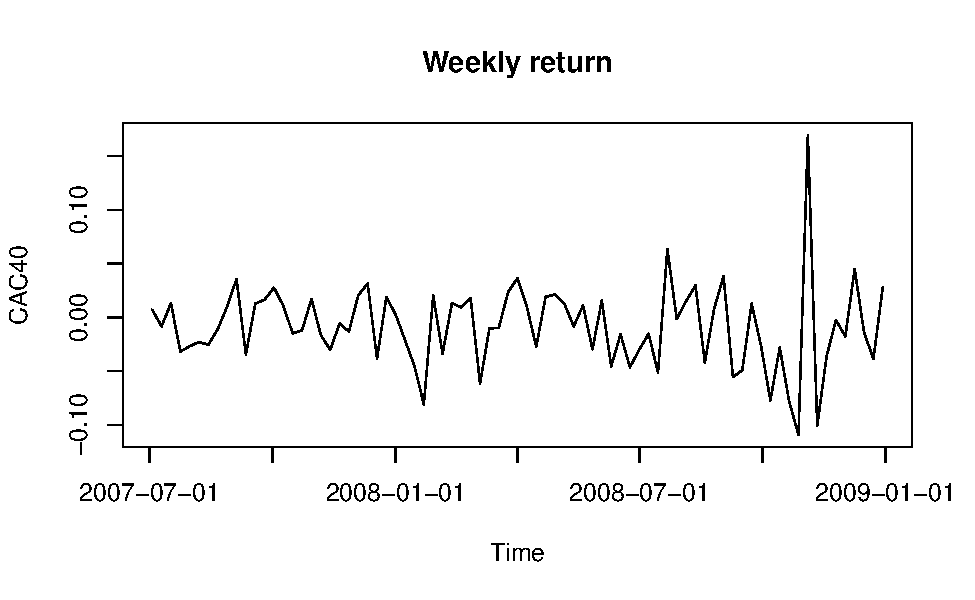
\includegraphics{TP1-Co_files/figure-latex/plot-cac-2-1.pdf}

\hypertarget{calcul-de-correlation}{%
\subsection{Calcul de correlation}\label{calcul-de-correlation}}

\begin{itemize}
\item
  Calculer la matrice de corrélation des actions de l'indice.
\item
  Rechercher des actions fortement corrélées et d'autres qui semblent
  indépendantes. Justifier ces observations en considérant la nature des
  entreprises.
\item
  Choisir 3 titres, et reproduire la figure 3.5, page 35 du manuel de B.
  Pfaff. Commenter les résultats obtenus.
\end{itemize}

\hypertarget{analyse-en-composantes-principales}{%
\subsection{Analyse en composantes
principales}\label{analyse-en-composantes-principales}}

Les 6 premiers facteurs expliquent 80\% de la variance.

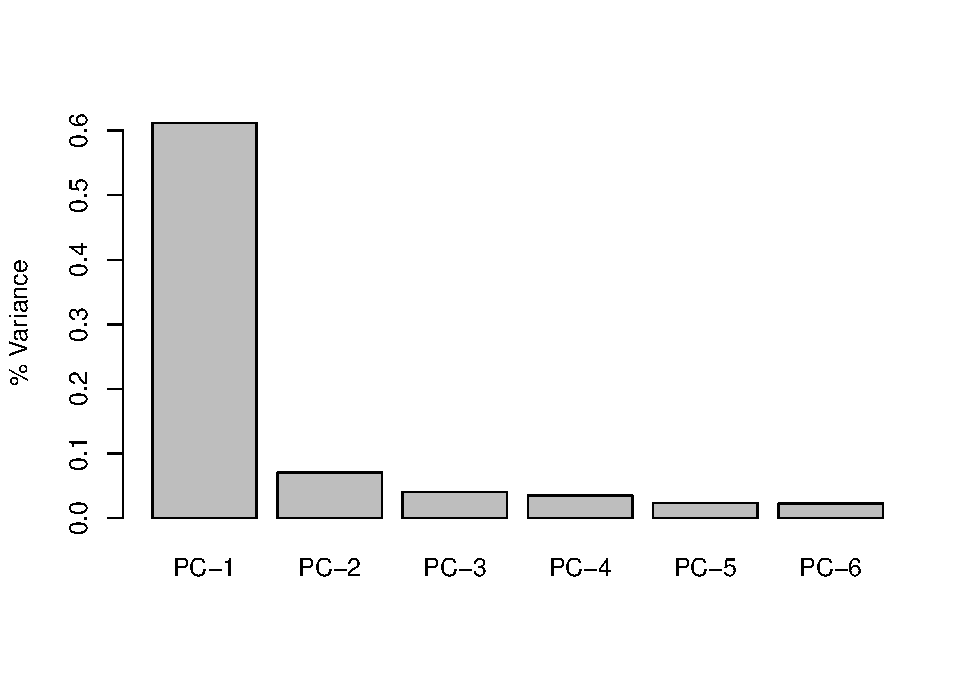
\includegraphics{TP1-Co_files/figure-latex/unnamed-chunk-3-1.pdf}

Les actions du CAC40 sont assez uniformement exposées au premier
facteur, que l'on peut de ce fait interpréter comme le ``marché''

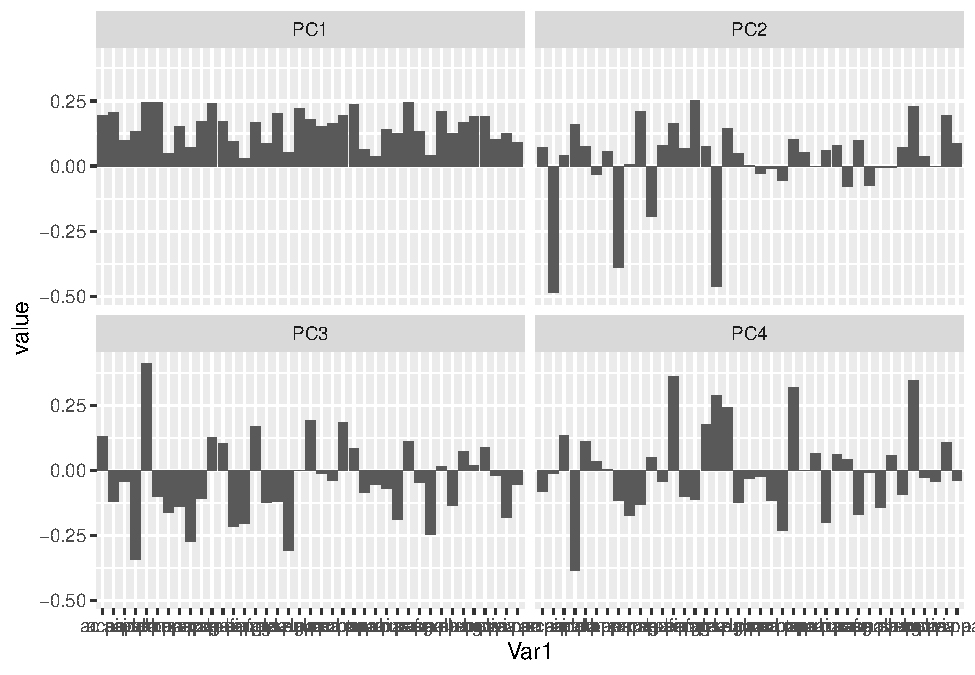
\includegraphics{TP1-Co_files/figure-latex/unnamed-chunk-4-1.pdf}

Projection des rendements hebdomadaires sur le 4 premières composantes
principales\}

Cette interprétation est validée en construisant une serie chronologique
du facteur 1 et en la comparant à l'indice lui même

\begin{Shaded}
\begin{Highlighting}[]
\NormalTok{  pc}\FloatTok{.1} \OtherTok{\textless{}{-}}\NormalTok{ ts.stocks }\SpecialCharTok{\%*\%}\NormalTok{ pca}\SpecialCharTok{$}\NormalTok{rotation[,}\DecValTok{1}\NormalTok{]}
\NormalTok{  ts.pc}\FloatTok{.1} \OtherTok{\textless{}{-}} \FunctionTok{timeSeries}\NormalTok{(pc}\FloatTok{.1}\NormalTok{, }\FunctionTok{time}\NormalTok{(ts.stocks))}
\end{Highlighting}
\end{Shaded}

\begin{Shaded}
\begin{Highlighting}[]
  \FunctionTok{plot}\NormalTok{(}\FunctionTok{cbind}\NormalTok{(}\FunctionTok{scale}\NormalTok{(ts.pc}\FloatTok{.1}\NormalTok{), }\FunctionTok{scale}\NormalTok{(ts.index)), }\AttributeTok{plot.type=}\StringTok{\textquotesingle{}single\textquotesingle{}}\NormalTok{,}
       \AttributeTok{col=}\FunctionTok{c}\NormalTok{(}\StringTok{\textquotesingle{}blue\textquotesingle{}}\NormalTok{, }\StringTok{\textquotesingle{}red\textquotesingle{}}\NormalTok{), }\AttributeTok{ylab=}\StringTok{\textquotesingle{}Rendement hebdomadaire normalisé\textquotesingle{}}\NormalTok{)}
  \FunctionTok{legend}\NormalTok{(}\StringTok{\textquotesingle{}bottomleft\textquotesingle{}}\NormalTok{, }\FunctionTok{c}\NormalTok{(}\StringTok{\textquotesingle{}PC 1\textquotesingle{}}\NormalTok{, }\StringTok{\textquotesingle{}CAC 40 index\textquotesingle{}}\NormalTok{), }\AttributeTok{lwd=}\DecValTok{2}\NormalTok{,}
         \AttributeTok{col=}\FunctionTok{c}\NormalTok{(}\StringTok{\textquotesingle{}blue\textquotesingle{}}\NormalTok{, }\StringTok{\textquotesingle{}red\textquotesingle{}}\NormalTok{), }\AttributeTok{cex=}\NormalTok{.}\DecValTok{6}\NormalTok{)}
\end{Highlighting}
\end{Shaded}

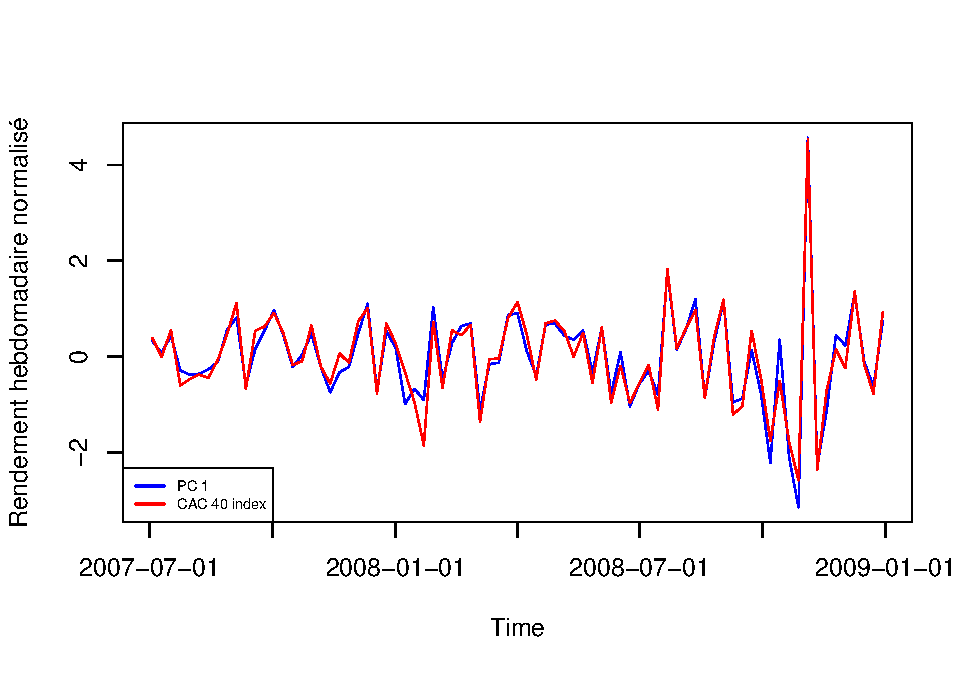
\includegraphics{TP1-Co_files/figure-latex/unnamed-chunk-6-1.pdf}

Rendement hebdomadaire de l'indice CAC 40 et premier facteur.

Les valeurs du secteur bancaire et des assurances se projettent
fortement sur la deuxième composante principale:

\begin{Shaded}
\begin{Highlighting}[]
\FunctionTok{print}\NormalTok{(}\FunctionTok{sort}\NormalTok{(}\FunctionTok{abs}\NormalTok{(pca}\SpecialCharTok{$}\NormalTok{rotation[,}\DecValTok{4}\NormalTok{])))}
\end{Highlighting}
\end{Shaded}

\begin{verbatim}
##       or.pa       bn.pa      san.pa      aca.pa       lr.pa       ug.pa 
## 0.001695215 0.004315204 0.007742585 0.012220467 0.024500716 0.028355637 
##       lg.pa      alu.pa      viv.pa      rno.pa       ul.pa       dg.pa 
## 0.030832473 0.033267585 0.039850223 0.039977924 0.043727566 0.043788591 
##       cs.pa     solb.br       ri.pa      ora.pa       ac.pa       su.pa 
## 0.047367622 0.055351700 0.061702858 0.065769399 0.079708887 0.090892167 
##       ei.pa      vie.pa      alo.pa       en.pa      bnp.pa       mc.pa 
## 0.099408477 0.106552004 0.110514748 0.112681476 0.115056616 0.116647458 
##      ker.pa      cap.pa       ai.pa      sgo.pa      saf.pa       ca.pa 
## 0.122288382 0.130958408 0.134899273 0.143647538 0.167832082 0.173012697 
##       fp.pa      pub.pa       ml.pa      gsz.pa      gle.pa       mt.pa 
## 0.177486858 0.199768799 0.230443630 0.241905440 0.285629669 0.316588220 
##      tec.pa      edf.pa      air.pa 
## 0.344043611 0.359656442 0.382942523
\end{verbatim}

\begin{Shaded}
\begin{Highlighting}[]
\FunctionTok{print}\NormalTok{(}\FunctionTok{sort}\NormalTok{(pca}\SpecialCharTok{$}\NormalTok{rotation[,}\DecValTok{4}\NormalTok{]))}
\end{Highlighting}
\end{Shaded}

\begin{verbatim}
##       air.pa        ml.pa       pub.pa        ca.pa       saf.pa       sgo.pa 
## -0.382942523 -0.230443630 -0.199768799 -0.173012697 -0.167832082 -0.143647538 
##       cap.pa       ker.pa        mc.pa       bnp.pa        en.pa        ei.pa 
## -0.130958408 -0.122288382 -0.116647458 -0.115056616 -0.112681476 -0.099408477 
##        su.pa        ac.pa        dg.pa        ul.pa       viv.pa        lg.pa 
## -0.090892167 -0.079708887 -0.043788591 -0.043727566 -0.039850223 -0.030832473 
##        ug.pa        lr.pa       aca.pa       san.pa        or.pa        bn.pa 
## -0.028355637 -0.024500716 -0.012220467 -0.007742585 -0.001695215  0.004315204 
##       alu.pa       rno.pa        cs.pa      solb.br        ri.pa       ora.pa 
##  0.033267585  0.039977924  0.047367622  0.055351700  0.061702858  0.065769399 
##       vie.pa       alo.pa        ai.pa        fp.pa       gsz.pa       gle.pa 
##  0.106552004  0.110514748  0.134899273  0.177486858  0.241905440  0.285629669 
##        mt.pa       tec.pa       edf.pa 
##  0.316588220  0.344043611  0.359656442
\end{verbatim}

On peut donc interpréter ce deuxième axe comme un facteur de rendement
spécifique au secteur ``bancassurance'', qui est un élément original du
paysage bancaire Français.

\end{document}
